\textbf{Pour cette première partie, aucune justification n'est demandée et une seule réponse est possible par question. Pour chaque question, reportez son numéro sur votre copie et indiquez votre réponse.}\\
Une réponse fausse ou l'absence de réponse n'enlève aucun point.


\subsection*{Question 1}
Une forme factorisée de l'expression $9x^2 - \dfrac{1}{9}$ est

\begin{tblr}{@{}XX}
	\textbf{A.}\quad $\left(3x - \dfrac{1}{3}\right)^2$ &
	\textbf{B.}\quad $\left(3x - \dfrac{1}{3}\right)\left(3x + \dfrac{1}{3}\right)$ \\
	\textbf{C.}\quad $\left(9x - \dfrac{1}{3}\right)^2$ &
	\textbf{D.}\quad $\left(9x - \dfrac{1}{3}\right)\left(9x + \dfrac{1}{3}\right)$
\end{tblr}

\subsection*{Question 2}
On considère la relation $E = \dfrac{x - y}{zt}$.

Lorsque $x = 3$, $y = -2$, $z = -3$, $t = -4$, on a :

\begin{tblr}{@{}XXXX}
	\textbf{A.}\quad $E = \dfrac{1}{12}$ &
	\textbf{B.}\quad $E = -\dfrac{5}{12}$ &
	\textbf{C.}\quad $E = \dfrac{5}{12}$ &
	\textbf{D.} $E = -\dfrac{1}{12}$
\end{tblr}

\subsection*{Question 3}
\begin{minipage}{0.42\linewidth}
	On considère une fonction $f$ définie sur l'intervalle $[-5 ; 9]$.

	On a représenté ci-contre sa courbe représentative dans un repère orthogonal.

	On note \quad $A = \dfrac{f(-4)}{f(-1)}$\,.

	Laquelle de ces propositions est vraie ?
\end{minipage}
\hfill
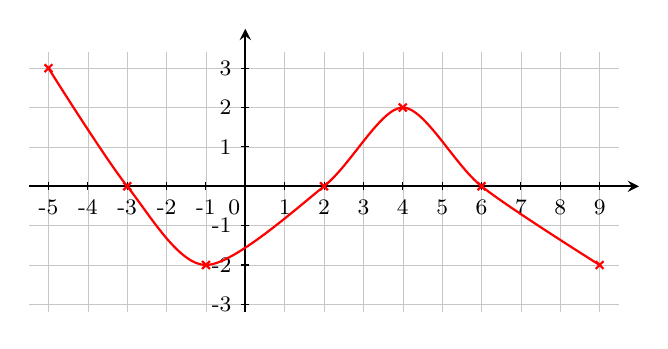
\begin{tikzpicture}[x=5mm,y=5mm,baseline={(current bounding box.center)},> = stealth]
	\draw[gray!45,very thin,xstep=1,ystep=1] (-5.5,-3.2) grid (9.5,3.4);
	\draw[thick,->] (-5.5,0)--(10,0);
	\draw[thick,->] (0,-3.2)--(0,4);
	\foreach \x in {-5,...,-1,1,2,...,9}
	{\draw (\x,1.5pt)--(\x,-1.5pt) node[below,font=\footnotesize]{\np{\x}};}
	\foreach \y in {-3,-2,-1,1,2,3}{\draw (1.5pt,\y)--(-1.5pt,\y) node[left,font=\footnotesize]{\np{\y}};}
	\node[below,font=\footnotesize] at (-4pt,-1.5pt) {0};
	\draw[red,thick,smooth, mark=x] plot coordinates {(-5,3) (-3,0) (-1,-2) (2,0) (4,2) (6,0) (9,-2)};
\end{tikzpicture}

\begin{tblr}{@{}XX}
	\textbf{A.}\quad $A = 0$ & \textbf{B.}\quad $A < 0$ \\[0.5em]
	\textbf{C.}\quad $A > 0$ & \textbf{D.}\quad On ne peut pas connaître le signe de $A$.
\end{tblr}

\subsection*{Question 4}


On considère l'inéquation sur $\R$
\[
(I) \quad -2x + 2 \geqslant 0.
\]
On note $S$ l'ensemble des solutions de l'inéquation $(I)$.

On peut affirmer que

\begin{tblr}{@{}XXXX}
	\textbf{A.}\quad $S = \left]-\infty ; 1\right]$ &
	\textbf{B.}\quad $S = \left[1 ; +\infty\right[$ &
	\textbf{C.}\quad $S = \left[-1 ; +\infty\right[$ &
	\textbf{D.}\quad $S = \left]-\infty ; -1\right]$
\end{tblr}

\subsection*{Question 5}
On considère ci-dessous le tableau de signes d'une fonction $f$ définie sur $\R$.

\begin{center}
	\begin{tblr}{colspec={|c|*{6}{X[c,8mm]}|},row{2}={8mm}}
		\hline
		$x$ & $-\infty$ & & $-3$ & & $2$ & $+\infty$ \\
		\hline
		Signe de $f(x)$ & & $+$ & $0$ & $-$ & $0$ & $+$ \\
		\hline
	\end{tblr}
\end{center}

Une expression possible de $f(x)$ est

\begin{tblr}{@{}XX}
	\textbf{A.}\quad $f(x) = (x+3)(2-x)$ & \textbf{B.}\quad $f(x) = (x+2)(x-3)$ \\
	\textbf{C.}\quad $f(x) = (x-2)(x+3)$ & \textbf{D.}\quad $f(x) = (x+2)(3+x)$
\end{tblr}

\subsection*{Question 6}
Le prix d'un article baisse de 50\,\% puis augmente de 40\,\%.

Ces deux variations sont équivalentes à

\begin{tblr}{@{}XX}
	\textbf{A.}\quad une baisse de 0\,\% & \textbf{B.}\quad une baisse de 70\,\% \\
	\textbf{C.}\quad une baisse de 10\,\% & \textbf{D.}\quad une baisse de 30\,\%
\end{tblr}



\subsection*{Question 7}


On s'intéresse aux adhérents d'une association.

On sait que 40\,\% d'entre eux sont des hommes et qu'il y a 30 femmes.

Le nombre total d'adhérents de cette association est égal à

\begin{tblr}{@{}XXXX}
	\textbf{A.}\quad 70 & \textbf{B.}\quad 40 & \textbf{C.}\quad 75 & \textbf{D.}\quad 50
\end{tblr}

\subsection*{Question 8}
On considère un réel $a$ quelconque, différent de 0.

Une seule de ces égalités est vraie. Laquelle ?

\begin{tblr}{@{}XXXX}
	\textbf{A.}\quad $\dfrac{a^8}{a^{-5}} = a^3$ &
	\textbf{B.}\quad $\dfrac{a^{30}}{a^2} = a^{15}$ &
	\textbf{C.}\quad $\left(a^{10}\right)^3 = a^{13}$ &
	\textbf{D.}\quad $\dfrac{a \times a^5}{a^2} = a^4$
\end{tblr}
